%!TEX root = ../main.tex
\newcommand{\body}{\ensuremath{\t{body}}\xspace}
\newcommand{\strokewidth}{\ensuremath{\t{stroke\_w}}\xspace}
\newcommand{\segmentationpoints}{\ensuremath{\t{sps}}\xspace}
\newcommand{\segmentationpoint}{\ensuremath{\t{sp}}\xspace}
\newcommand{\image}{\ensuremath{\t{image}}\xspace}
\newcommand{\subimage}{\ensuremath{\t{sub\_image}}\xspace}
\newcommand{\leftsubimage}{\ensuremath{\t{left}}\xspace}
\newcommand{\rightsubimage}{\ensuremath{\t{right}}\xspace}
\newcommand{\segmentfurther}{\ensuremath{\t{todo}}\xspace}
\newcommand{\characters}{\ensuremath{\t{done}}\xspace}
\newcommand{\parameters}{\ensuremath{\t{parameters}}\xspace}

\begin{figure}
	%!TEX root = ../main.tex
\MakeRobust{\Call}

\newcommand{\body}{\ensuremath{\mathit{body}}\xspace}
\newcommand{\strokewidth}{\ensuremath{\mathit{stroke\_w}}\xspace}
\newcommand{\segmentationpoints}{\ensuremath{\mathit{sps}}\xspace}
\newcommand{\segmentationpoint}{\ensuremath{\mathit{sp}}\xspace}
\newcommand{\image}{\ensuremath{\mathit{image}}\xspace}
\newcommand{\subimage}{\ensuremath{\mathit{sub\_image}}\xspace}
\newcommand{\leftsubimage}{\ensuremath{\mathit{left}}\xspace}
\newcommand{\rightsubimage}{\ensuremath{\mathit{right}}\xspace}
\newcommand{\segmentfurther}{\ensuremath{\mathit{todo}}\xspace}
\newcommand{\characters}{\ensuremath{\mathit{done}}\xspace}
\newcommand{\parameters}{\ensuremath{\mathit{parameters}}\xspace}

\begin{algorithmic}[1]
\Function{segment}{$\image,\, \parameters$}
\State \body $\gets$ \Call{body\_region}{\image}
\State \strokewidth $\gets$ \Call{stroke\_width}{\image} 
\item[]
\State \segmentationpoints $\gets$ \Call{segmentation\_points}{\body, \strokewidth} 
\State \segmentfurther \characters $\gets$ [\image], []
\item[]
\While{\Call{continue}{~}}
	\State $\subimage \gets$ \Call{select\_sub\_image}{\segmentfurther} 
	\State $\segmentationpoint \gets$ \Call{select\_sp}{\segmentationpoints} 
	\State \leftsubimage, \rightsubimage $\gets$ \Call{split}{\subimage, \segmentationpoint}
	%
   \If {\Call{is\_character}{\leftsubimage}}
      \State \Call{add}{\leftsubimage, \characters}
   \Else
		\State \Call{add}{\leftsubimage, \segmentfurther}
   \EndIf \Comment{Repeat for \rightsubimage.}
\EndWhile
\State \textbf{return} \Call{merge}{\segmentfurther, \characters}
\EndFunction
\end{algorithmic}
	\caption{Binary Over Segmentation Algorithm.}
	\label{alg:method:segmentation:algorithm}
\end{figure}

We use binary over segmentation to segment the words into images, the pseudo code of this algorithm is presented in \cref{alg:method:segmentation:algorithm}. This algorithm aims to segment an image into two sub-images on the segmentation point that is most likely. One of these sub images is then selected and segmented again into two new sub-images, if it is not a character. This is repeated until the termination condition has been reached, i.e. \function{continue}{} is not longer true. If the segmentation has finished the list with images that could be segmented further, \segmentfurther, and the list with characters, \characters, are merged by \function{merge}. This function ensures that the final returned list of character images is in the same order as the characters occur in the word image. \Cref{fig:method:segmentation:tree} illustrates how the algorithm segments an images of a word into images of characters.

The \parameters passed to \function{segment}{} in \cref{alg:method:segmentation:algorithm} contain the maximum character length and the minimum, average and maximum image width and height. The maximum word length is the length of the longest word in the data set. The other six values are determined based on the data. Before computing the minimum, average or maximum all widths, or heights, that are not within two standard deviations of the mean of the character widths, or heights, are discarded as outliers. 

The different functions referenced in \cref{alg:method:segmentation:algorithm} are discussed in \crefrange{sss:method:segmentaton:bodyregion}{sss:method:segmentaton:segmentfurther}.

\begin{figure}
	\centering
	\timemachine{Create this image, as a tree with the word image as the root and the character image as the leaf. In the images mark the used segmentation line. Don't show left over segmentation lines in the leaves.}
	\missingfigure{Visualize how a word is segmented, using a tree view. Sort of like \cref{fig:introduction:binaryOversegmentation:chainfailure}.}
	\caption{Caption here}
	\label{fig:method:segmentation:tree}
\end{figure}

\subsubsection{Body Region}
\label{sss:method:segmentaton:bodyregion}
The body region is the part of the image that is between the lower and the upper base line. To compute the low base line for each column in the image the lowest row with a foreground pixel is computed. The low base line is the mode of the these rows. The high baseline is computed in the same way, but uses the highest row of each column with a foreground pixel. 

The part of the image between the low and high base line is the body region. Using this region for the computation of the segmentation points reduces the influence of extensive ligatures. \Cref{fig:method:segmentation:baseline} illustrates examples of the determination of the baselines. \Cref{fig:method:segmentation:baseline:succes} reflects the intended outcome, the second example, \cref{fig:method:segmentation:baseline:failure}, draws the upper baseline too high because of the extra curve on the last letter.

	\begin{figure}
		\centering
		\subfloat[]{
			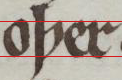
\includegraphics[width=0.45\columnwidth]{shared/img/method/base_line_succes.png}%
			\label{fig:method:segmentation:baseline:succes}%
		}
		\hspace{0.03\columnwidth}
		\subfloat[]{
			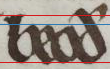
\includegraphics[width=0.45\columnwidth]{shared/img/method/base_line_fail.png}%
			\label{fig:method:segmentation:baseline:failure}%
		}
		\caption{An example of \protect\subref{fig:method:segmentation:baseline:succes} correct and \protect\subref{fig:method:segmentation:baseline:failure} incorrect baselines found with the described method. The found baselines are shown in red. If the found baselines were incorrect, the correct baselines are shown in blue.}
		\label{fig:method:segmentation:baseline}
	\end{figure}

\subsubsection{Stroke Width}
\label{sss:method:segmentaton:strokwidth}
\todo[inline]{What is the strokewidth}
\todo[inline]{How do we compute it}

\subsubsection{Segmentation Points}
\label{sss:method:segmentaton:segmentationpoints}
\todo[inline]{Computation, based on Fig 3 in old version}
\todo[inline]{Filtering SSP, subsubsection per filter method. Show results, succesful and failure.}

\subsubsection{Continue}
\label{sss:method:segmentaton:termination}
\todo[inline]{Wanneer stoppen we met ons lusje}
\todo[inline]{Waarom nemen we langste woord op basis van alle data, i.pv. alleen niet outliers.}

\subsubsection{Select Sub-Image}
\label{sss:method:segmentaton:selectsubimage}
\todo[inline]{How to select the next sub image}

\subsubsection{Select SP}
\label{sss:method:segmentaton:selectssp}
\todo[inline]{How to select the next SSP }

\subsubsection{Split}
\label{sss:method:segmentaton:splitimage}
\todo[inline]{How to split an image, compare our approach with the splitting along a straight line. Mention A* parameters.}

\subsubsection{Is Character}
\label{sss:method:segmentaton:segmentfurther}
\todo[inline]{How to determine if an image should be segmented further, or if it is an character.}